\documentclass{beamer}
 
\usepackage[utf8]{inputenc}
%\usepackage{fontspec}
%\setmainfont{Linux Libertine O}
%\fontfamily{Computer Modern}\selectfont{Computer Modern Serif}
%\newfontfamily\cmss
 
\usetheme{CambridgeUS} 
%Information to be included in the title page:
\title{Integração numérica: método de simpson}
\author[Mateus]
{Mateus Schroeder da Silva}

\institute{UDESC}
\date{06-2019}
 
%\logo{
\includegraphics[height=1cm]{images/marca-udesc.png}}
\begin{document}
 
\frame{\titlepage}
 
%\begin{frame}
%\frametitle{AA}
%This is a text in the first frame. This is a text in the first frame. This is a text in the first frame.
%\end{frame}

					
\begin{frame}
\frametitle{Derivação da fórmula de área}
Vamos considerar a área sob uma parábola genérica $y = ax^2 + bx + c$
Suporemos que o intervalo de integração é $[-h, +h]$ e $\Delta x = h$.
$$ \int_{-h}^h {(ax^2 + bx + c) dx}$$
$$ \left[ \dfrac{ax^3}{3} + \dfrac{bc^2}{2} + cx \right]_{-h}^{h} = \left( \dfrac{ah^3}{3} + \dfrac{bh^2}{2} + ch \right) -  \left( -\dfrac{ah^3}{3} + \dfrac{bh^2}{2} + -ch \right)$$
$$= \dfrac{2a^3}{3} + 2ch = \dfrac{h}{3} \left( 2ah^2 + 6c \right)$$
\end{frame}

\begin{frame}
\frametitle{}
$$x_0(-h, y_0), x_1(0,y_1), x_2(h, y_2)$$
Substituindo os pontos na equação genérica temos:
$$ y_0 = ah^2 - bh + c$$
$$y_1 = c$$
$$ y_2 = ah^2 + bh + c$$
Temos então adicionando a 1ª e 3ª linhas:
$$2ah^2 = y_0 - 2y_1 + y_2$$
\end{frame}
\begin{frame}
\frametitle{Derivação da fórmula de área}
Substituindo na fórmula da área:
$$A = \dfrac{2a^3}{3} + 2ch = \dfrac{h}{3} \left( 2ah^2 + 6c \right)$$
$$ = \dfrac{h}{3} \left( y_0 - 2y_1 + y_2 + 6c \right) $$
$$ = \dfrac{h}{3} \left( y_0 - 2y_1 + y_2 + 6y_1 \right) $$
$$ = \dfrac{h}{3} \left( y_0 + 4y_1 + y_2  \right) $$
\end{frame}
\begin{frame}
\frametitle{Derivação da fórmula de área}
Se continuássemos analogamente teríamos:
$$ = \dfrac{h}{3} \left( y_2 + 4y_3 + y_4  \right) $$
$$ = \dfrac{h}{3} \left( y_4 + 4y_5 + y_6  \right) $$
E a fórmula geral então:
$$ \int_{-h}^h f(x) \approx \dfrac{h}{3} \left( y_0 + 4y_1 + 2y_3 + \cdots + 4y_{n-1} + y_n  \right) $$
\end{frame}
\begin{frame}
	\begin{figure}[htb]
	\centering
    	    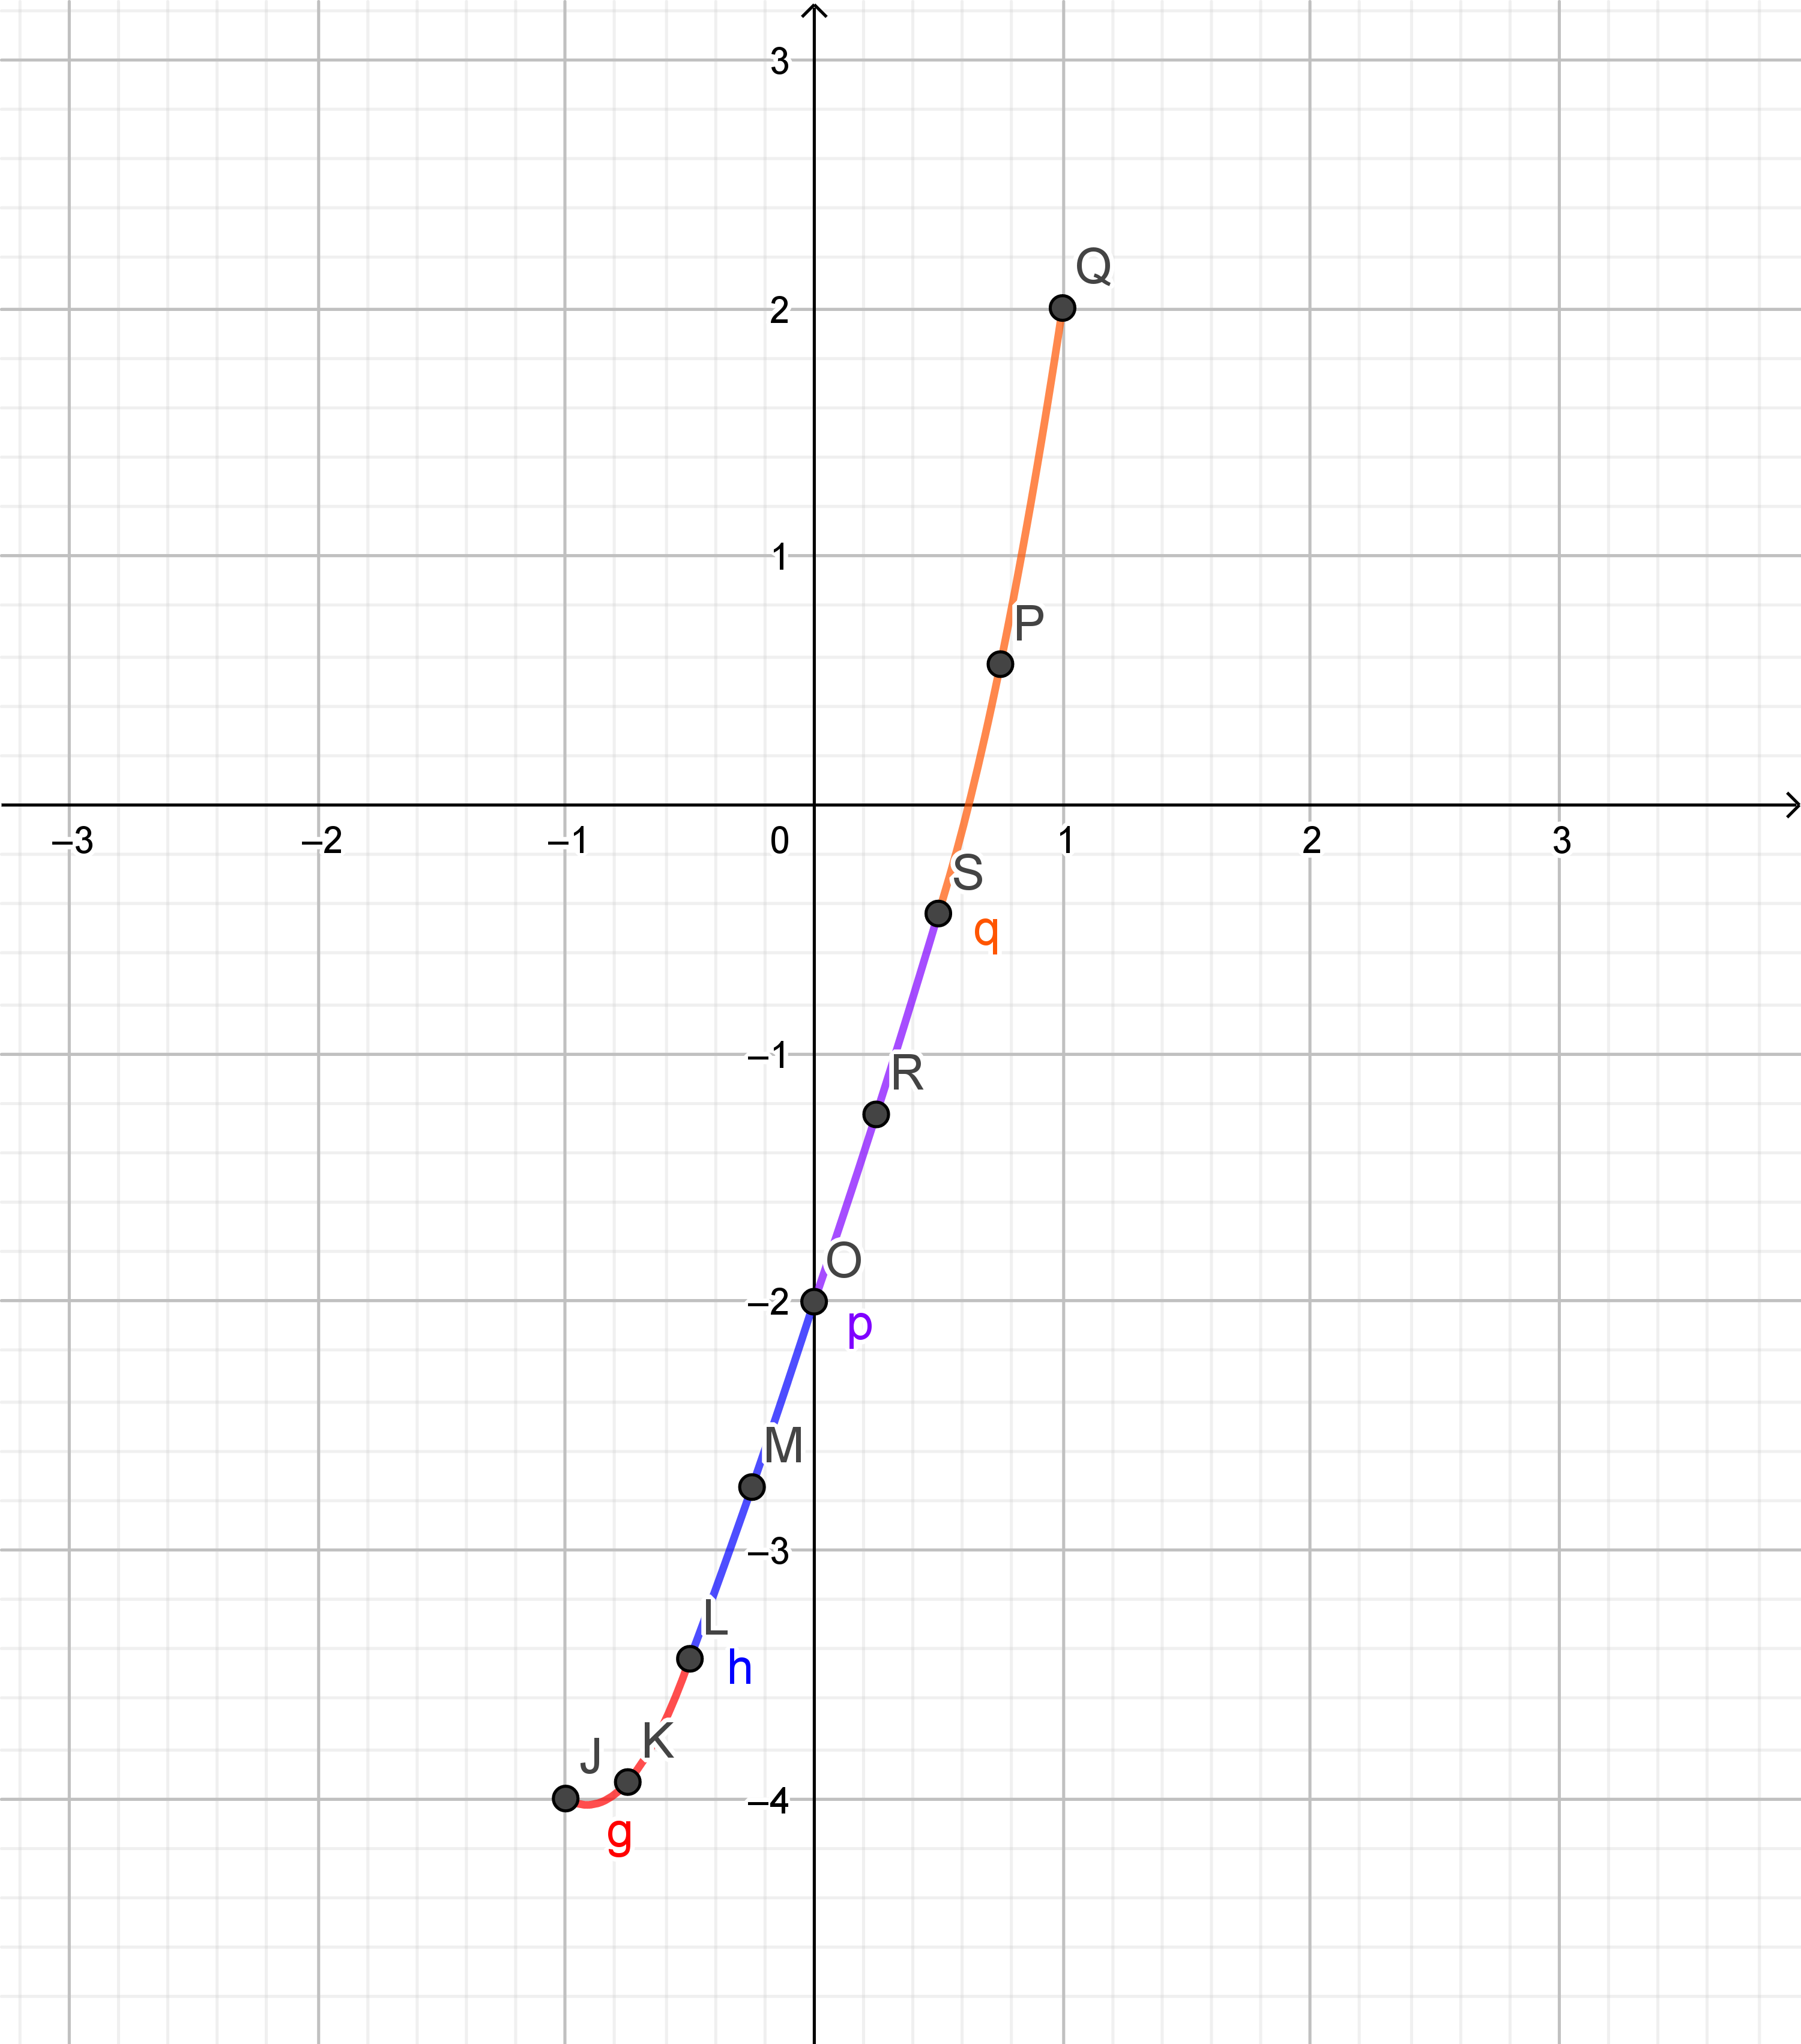
\includegraphics[width=8cm, height=5cm]{images/x1.png}
       	        \vspace{0.01em}
       	 \caption{$x^4 + 3x - 2$}
	\end{figure}
\end{frame}
\begin{frame}
	\begin{figure}[htb]
	\centering
    	    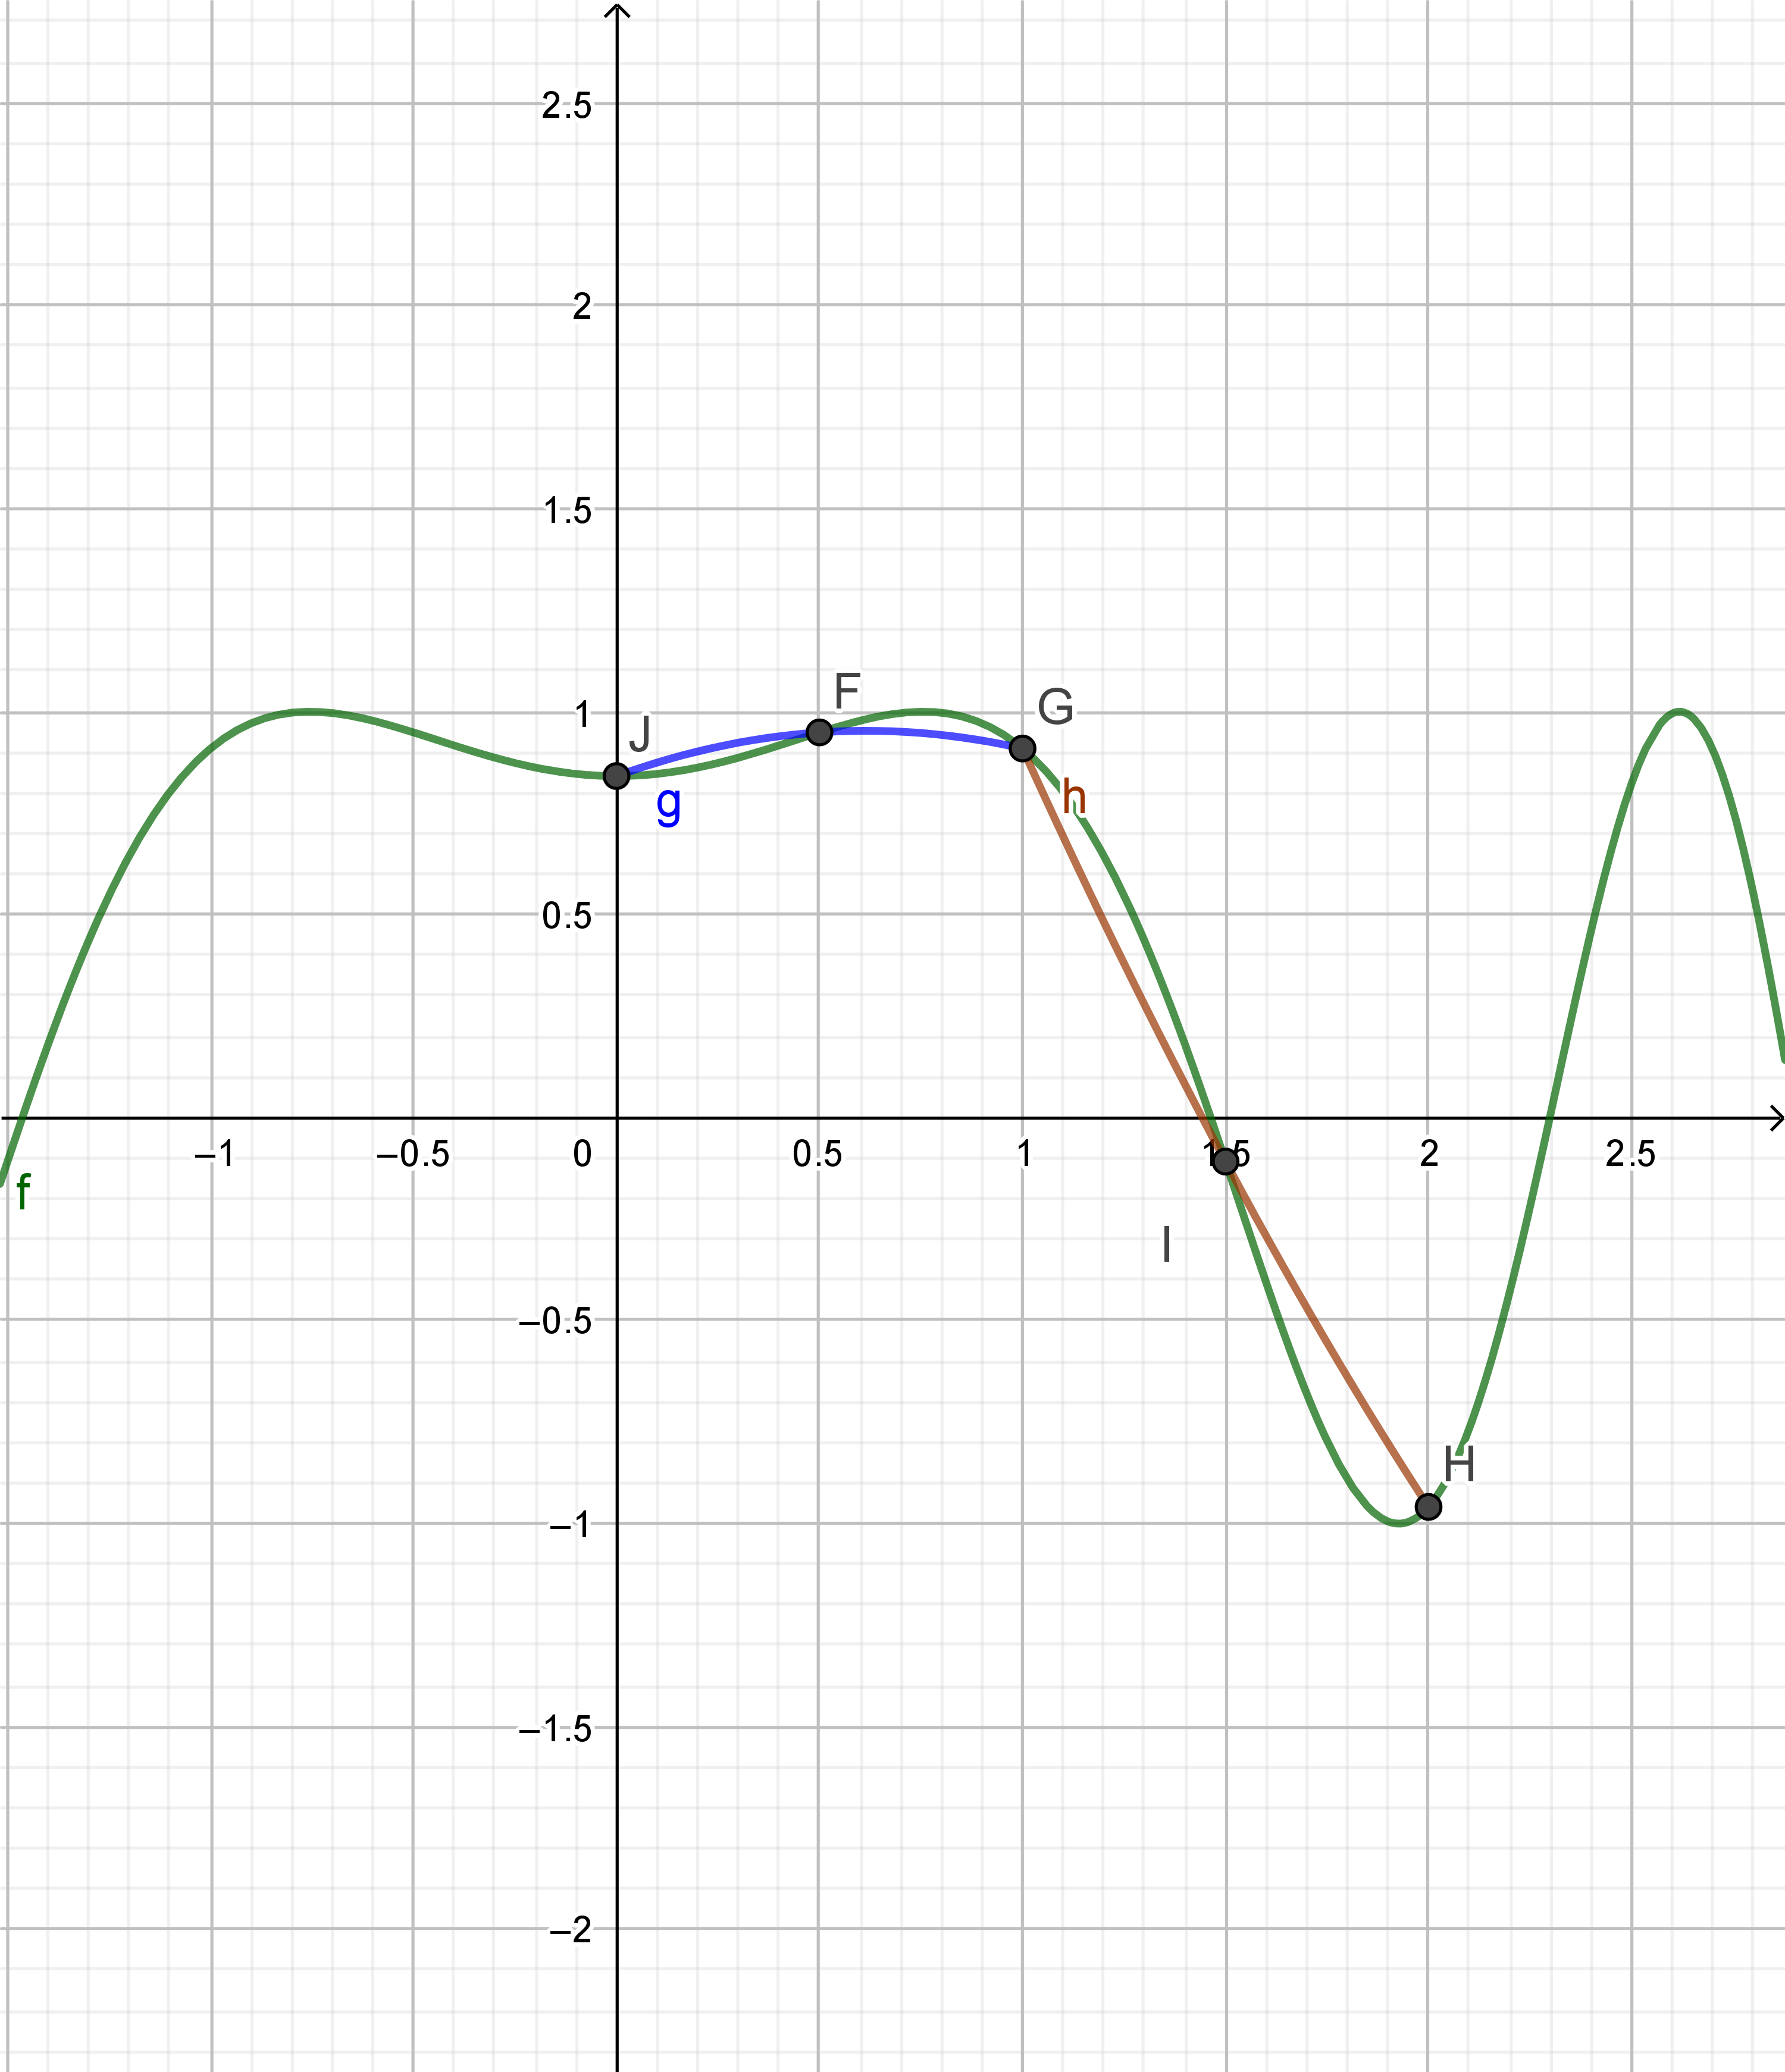
\includegraphics[width=8cm, height=5cm]{images/x2.png}
       	        \vspace{0.01em}
       	 \caption{$sin(x^2 + 1)$}
	\end{figure}
\end{frame}
\begin{frame}
	\begin{figure}[htb]
	\centering
    	    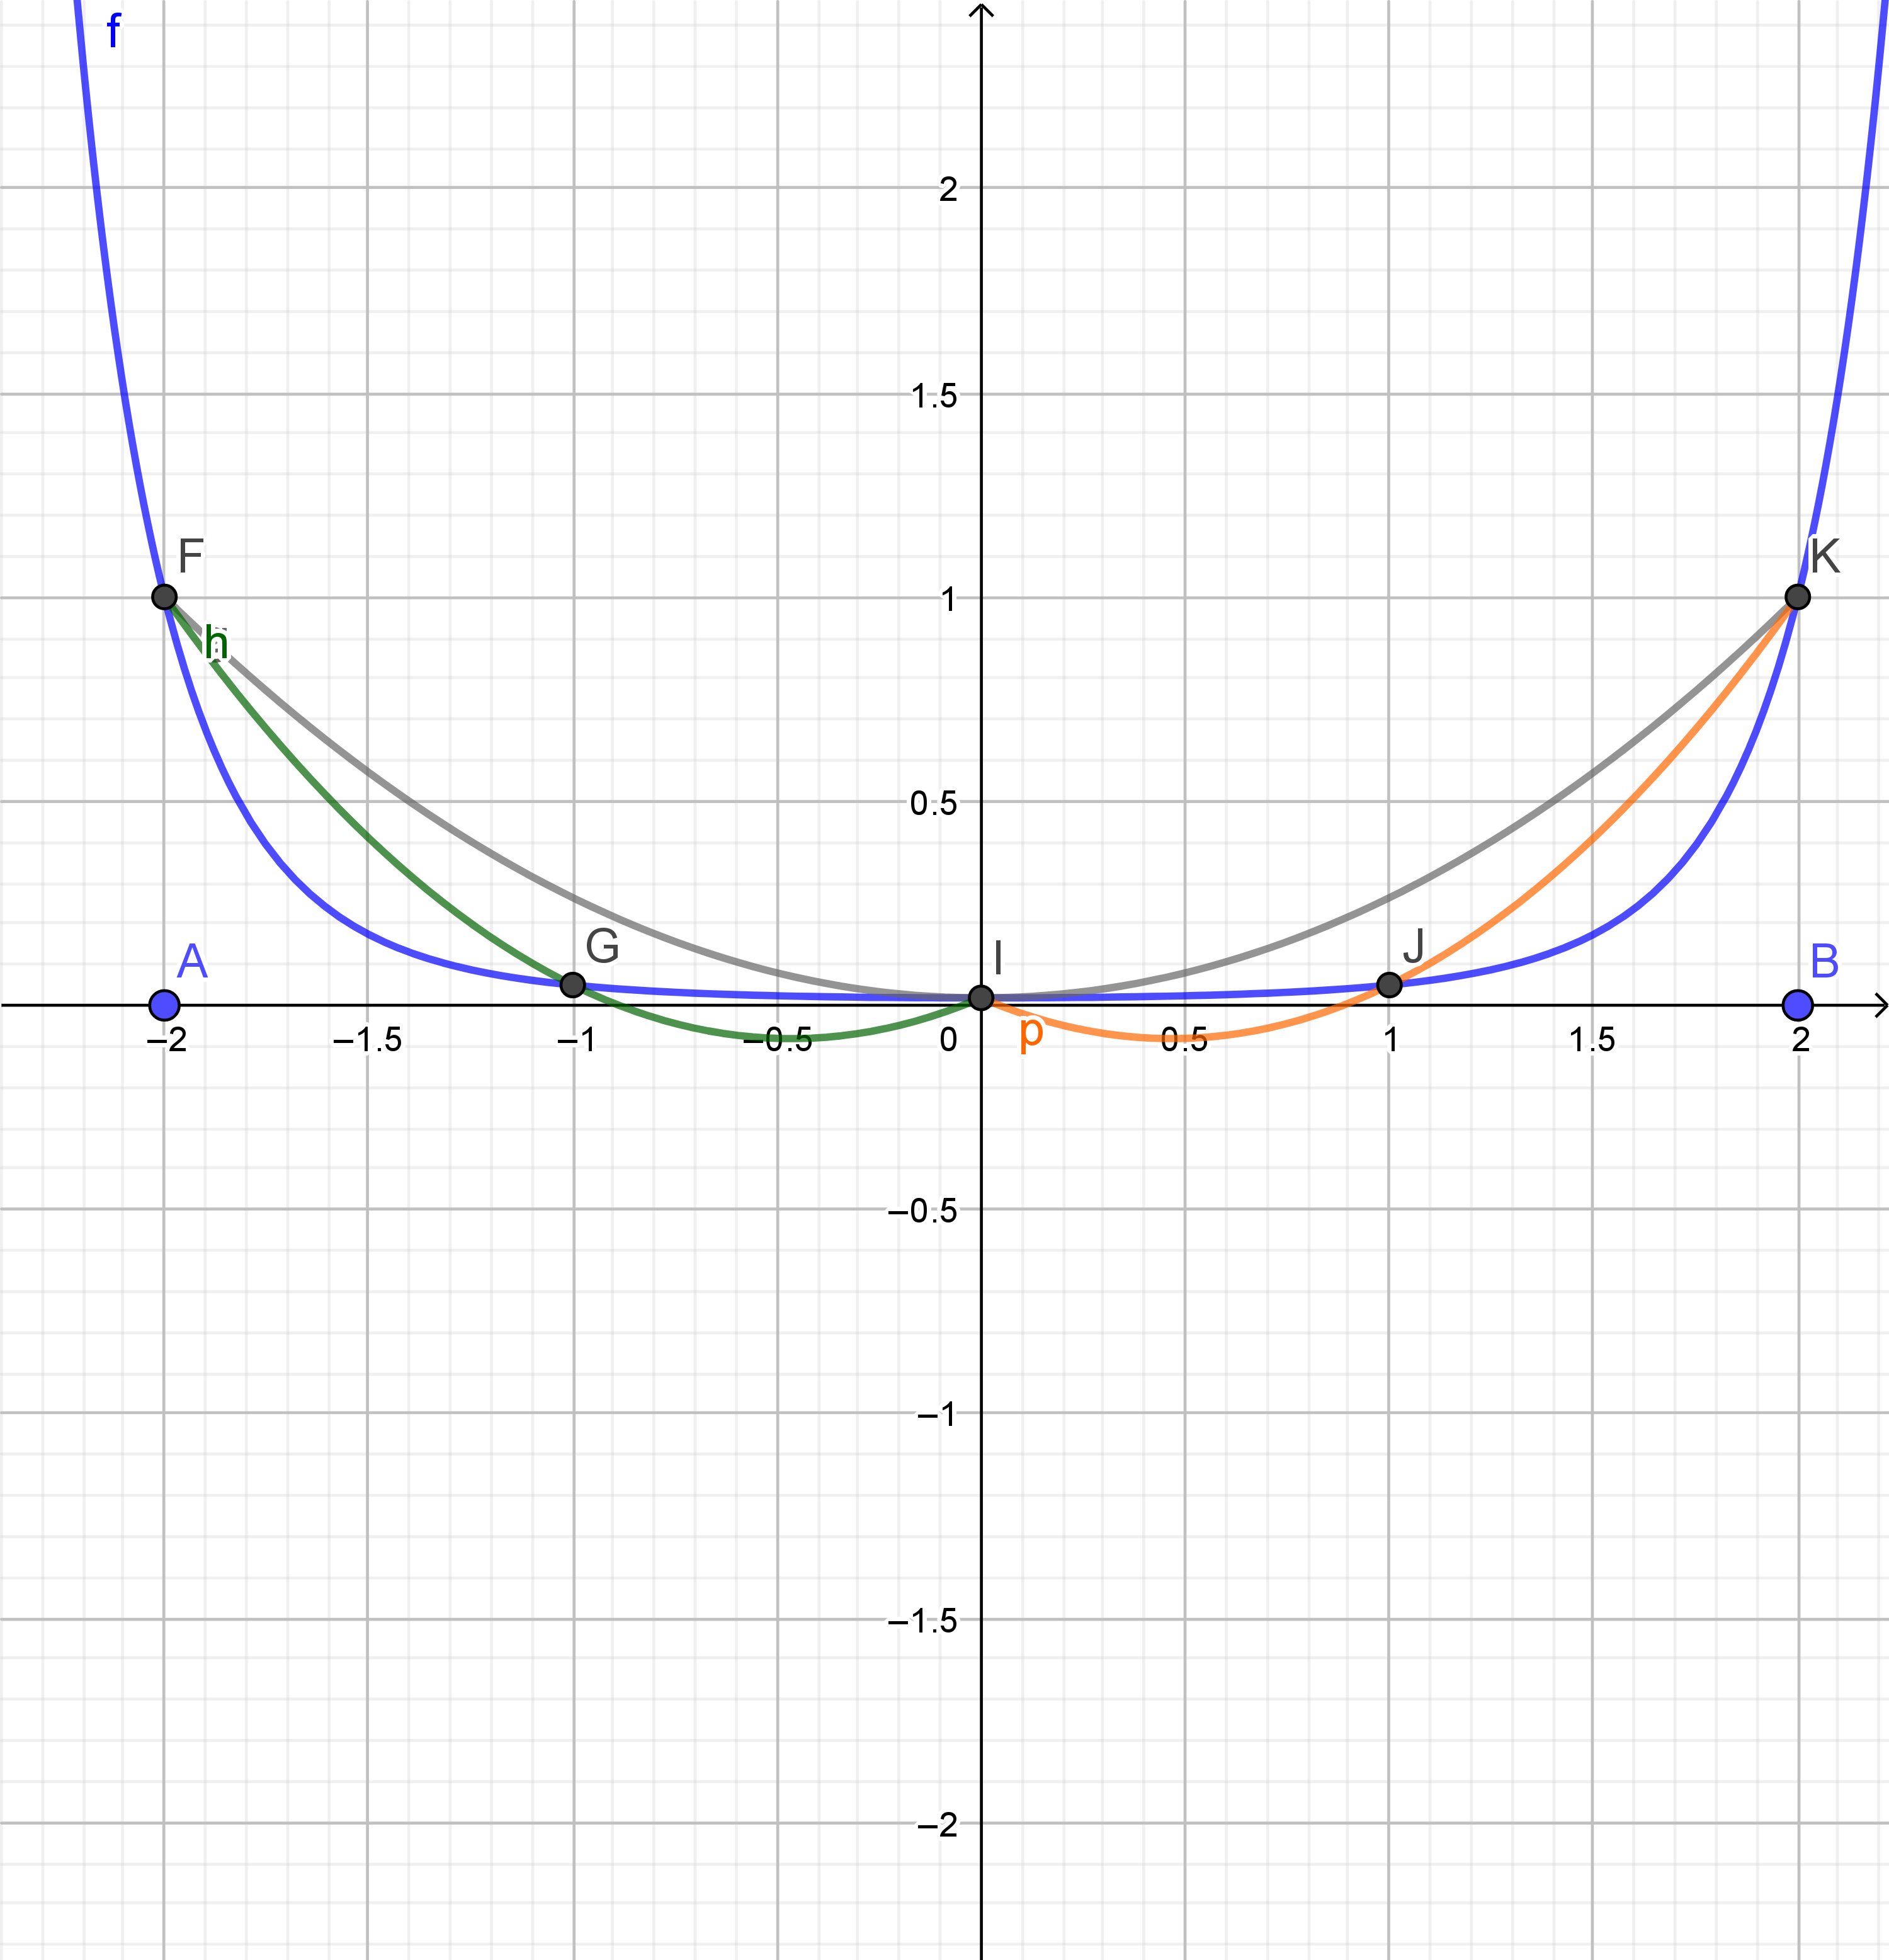
\includegraphics[width=8cm, height=5cm]{images/x3.png}
       	        \vspace{0.01em}
       	 \caption{$e^{x^2 -4}$}
	\end{figure}
\end{frame}
\begin{frame}
\frametitle{Referências}
https://www.intmath.com/integration/6-simpsons-rule.php
\end{frame}
%\begin{frame}
%\frametitle{Derivação da fórmula de área}
%\end{frame}
%\begin{frame}
%\frametitle{Derivação da fórmula de área}
%\end{frame}
\end{document}
